\documentclass[12pt,a4paper]{article}

% ============================================================
% PREAMBLE
% ============================================================
\usepackage{amsmath}
\usepackage{amssymb}
\usepackage{geometry}
\geometry{margin=2.5cm}
\usepackage{booktabs}
\usepackage{xcolor}
\usepackage{hyperref}
\usepackage{listings}
\usepackage{pgfplots}
\pgfplotsset{compat=1.18}
\usepackage[skins,breakable]{tcolorbox}
\usepackage{enumitem}
\usepackage{fancyhdr}
\usepackage{tikz}
\usepackage{array}

% ---- tcolorbox environments ----
\newtcolorbox{curiositybox}[1]{colback=yellow!10, colframe=orange!80!black, fonttitle=\bfseries, title=#1, breakable}
\newtcolorbox{infobox}[1]{colback=blue!5, colframe=blue!60!black, fonttitle=\bfseries, title=#1, breakable}
\newtcolorbox{mistakebox}[1]{colback=red!5, colframe=red!60!black, fonttitle=\bfseries, title=#1, breakable}
\newtcolorbox{learnbox}[1]{colback=green!5, colframe=green!60!black, fonttitle=\bfseries, title=#1, breakable}

% ---- lstlisting configuration ----
\lstset{language=Python, basicstyle=\ttfamily\small, keywordstyle=\color{blue},
        commentstyle=\color{gray}, stringstyle=\color{red},
        showstringspaces=false, breaklines=true, frame=single}

% ---- fancyhdr ----
\pagestyle{fancy}
\fancyhf{}
\lhead{Topic 15: Singularities}
\rhead{Unit II --- Complex Variables}
\cfoot{\thepage}

% ---- title ----
\title{\textbf{Topic 15: Singularities}\\[6pt]
       \large Unit II --- Complex Variable: Integration\\[4pt]
       \normalsize Complex Variables and Special Functions\\
       JNTUA College of Engineering (Autonomous)}
\author{}
\date{}

% ============================================================
\begin{document}
% ============================================================
\maketitle
\tableofcontents
\newpage

% ============================================================
\section{Opening Hook}
% ============================================================
\begin{curiositybox}{Hook}
Analytic functions are beautifully smooth --- until they suddenly fail to be analytic at certain
points. Those exceptional points are singularities, and the way a function misbehaves there tells
us almost everything we need for later contour-integration techniques.
\end{curiositybox}

% ============================================================
\section{What Is a Singularity?}
% ============================================================

A function $f(z)$ that is analytic throughout a region $D$ is well-behaved at every point of $D$.
But many functions of practical interest fail to be analytic at one or more isolated points.
Understanding the nature of those failures is the subject of this topic.

\begin{infobox}{Singular Point and Isolated Singularity}
\textbf{Singular point.}
A point $z = z_0$ is called a \emph{singular point} (or \emph{singularity}) of $f(z)$ if $f$ is
\emph{not} analytic at $z_0$.

\textbf{Isolated singularity.}
The point $z_0$ is an \emph{isolated singularity} of $f(z)$ if there exists some $\delta > 0$ such
that $f$ is analytic in the punctured disk
\[
  0 < |z - z_0| < \delta,
\]
but not analytic at $z_0$ itself.

In other words, $z_0$ is ``surrounded'' by a region of analyticity; it is the only singular point
in some neighbourhood of itself.

\textbf{Non-isolated singularity.}
If every neighbourhood of $z_0$ contains another singular point, then $z_0$ is a
\emph{non-isolated singularity}. (Example: $\operatorname{Log}(z)$ has a branch cut, an entire
ray of non-isolated singularities.)

For this topic we focus entirely on \emph{isolated} singularities.
\end{infobox}

\begin{center}
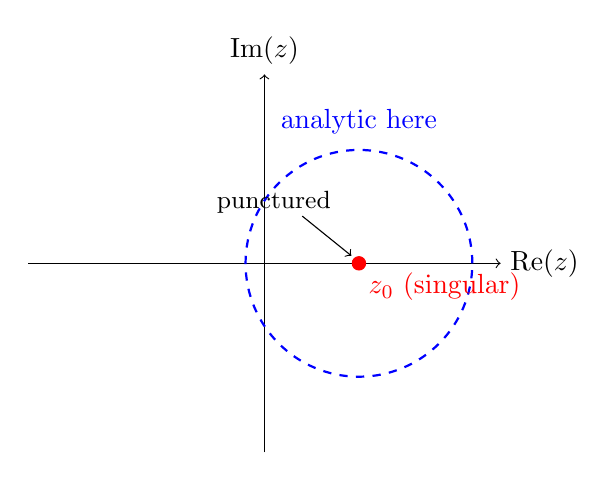
\begin{tikzpicture}[scale=1.2]
  % axes
  \draw[->] (-2.5,0) -- (2.5,0) node[right] {$\operatorname{Re}(z)$};
  \draw[->] (0,-2) -- (0,2) node[above] {$\operatorname{Im}(z)$};
  % punctured disk
  \draw[dashed, blue, thick] (1,0) circle (1.2cm);
  % singular point
  \filldraw[red] (1,0) circle (2pt) node[below right] {$z_0$ (singular)};
  % analytic region label
  \node[blue] at (1,1.5) {analytic here};
  % puncture label
  \draw[->] (0.4,0.5) -- (0.92,0.08);
  \node at (0.1,0.65) {\small punctured};
\end{tikzpicture}
\end{center}

\begin{learnbox}{Key Takeaway}
An isolated singularity is a lone bad point surrounded by a disk of analyticity.
Every isolated singularity falls into exactly one of three types: removable, pole, or essential.
\end{learnbox}

% ============================================================
\section{Classification of Isolated Singularities}
% ============================================================

The three types are distinguished by what happens to $\lim_{z\to z_0} f(z)$ and by the structure
of the Laurent series of $f$ in the punctured disk $0 < |z - z_0| < \delta$.

\begin{infobox}{Three Types of Isolated Singularity}
Let $z_0$ be an isolated singularity of $f(z)$, and let
\[
  f(z) = \sum_{n=-\infty}^{\infty} c_n (z-z_0)^n
\]
be its Laurent series in $0 < |z-z_0| < \delta$.

\begin{center}
\renewcommand{\arraystretch}{1.4}
\begin{tabular}{>{\bfseries}l l l}
\toprule
Type & Principal part & Limit behaviour \\
\midrule
Removable & No negative-power terms ($c_n = 0$ for $n < 0$) & $\lim_{z\to z_0} f(z)$ exists (finite) \\
Pole of order $m$ & Finitely many negative powers, lowest $c_{-m}(z-z_0)^{-m}$, $c_{-m}\neq 0$ & $\lim_{z\to z_0}|f(z)| = \infty$ \\
Essential & Infinitely many negative-power terms & Limit does not exist (Weierstrass) \\
\bottomrule
\end{tabular}
\end{center}

A pole of order $m=1$ is called a \emph{simple pole}.
\end{infobox}

\begin{learnbox}{Intuition}
Think of a removable singularity as a ``hole'' that can be patched, a pole as a spike that blows
up in a controlled algebraic way, and an essential singularity as chaotic blow-up with no pattern.
\end{learnbox}

% ============================================================
\section{Removable Singularities}
% ============================================================

\begin{infobox}{Definition and Criterion}
$z_0$ is a \emph{removable singularity} of $f$ if
\[
  \lim_{z \to z_0} (z - z_0)\, f(z) = 0.
\]
Equivalently, $\lim_{z\to z_0} f(z) = L$ for some finite $L$.  
If we \emph{define} $f(z_0) = L$, the extended function is analytic at $z_0$ --- the singularity
is ``removed.''

The Laurent series of $f$ about $z_0$ contains \emph{no negative powers}:
\[
  f(z) = c_0 + c_1(z-z_0) + c_2(z-z_0)^2 + \cdots
\]
\end{infobox}

\textbf{Classic example.}
$f(z) = \dfrac{\sin z}{z}$ at $z = 0$.

Expanding $\sin z$:
\[
  \frac{\sin z}{z} = \frac{1}{z}\!\left(z - \frac{z^3}{3!} + \frac{z^5}{5!} - \cdots\right)
  = 1 - \frac{z^2}{6} + \frac{z^4}{120} - \cdots
\]
No negative powers $\Rightarrow$ removable singularity at $z = 0$.

\begin{learnbox}{Key Takeaway}
A removable singularity appears because the numerator and denominator vanish to the same order.
Cancellation leaves a finite limiting value.
\end{learnbox}

% ============================================================
\section{Poles}
% ============================================================

\begin{infobox}{Simple Pole and Pole of Order $m$}
$z_0$ is a \textbf{pole of order $m$} ($m \geq 1$, $m \in \mathbb{Z}$) if $f(z)$ can be written as
\[
  f(z) = \frac{g(z)}{(z - z_0)^m},
\]
where $g(z)$ is analytic at $z_0$ and $g(z_0) \neq 0$.

The Laurent series of $f$ about $z_0$ has the form
\[
  f(z) = \frac{c_{-m}}{(z-z_0)^m} + \frac{c_{-m+1}}{(z-z_0)^{m-1}} + \cdots + \frac{c_{-1}}{z-z_0}
         + c_0 + c_1(z-z_0) + \cdots,
\]
with $c_{-m} \neq 0$. The terms with negative powers form the \emph{principal part}.

\textbf{Simple pole}: $m = 1$, so the principal part is just $\dfrac{c_{-1}}{z - z_0}$.

\textbf{Connection to denominator zeros.}
If $f(z) = p(z)/q(z)$ with $q(z_0) = 0$ but $p(z_0) \neq 0$, and $q$ has a zero of order $m$ at
$z_0$, then $f$ has a pole of order $m$ at $z_0$.
\end{infobox}

\begin{learnbox}{Key Takeaway}
A pole is an algebraic blow-up: as $z \to z_0$ from any direction, $|f(z)| \to \infty$ at a rate
controlled by the order $m$. The order equals the multiplicity of the zero in the denominator
(after cancelling any shared factors with the numerator).
\end{learnbox}

% ============================================================
\section{Essential Singularities}
% ============================================================

\begin{infobox}{Definition and Weierstrass Theorem}
$z_0$ is an \textbf{essential singularity} of $f$ if the Laurent series in $0 < |z-z_0|<\delta$
contains \emph{infinitely many negative-power terms}:
\[
  f(z) = \cdots + \frac{c_{-3}}{(z-z_0)^3} + \frac{c_{-2}}{(z-z_0)^2} + \frac{c_{-1}}{z-z_0}
         + c_0 + c_1(z-z_0) + \cdots
\]

\textbf{Weierstrass--Casorati Theorem.}
If $z_0$ is an essential singularity, then for every punctured neighbourhood of $z_0$, the image
$f\!\left(\{0<|z-z_0|<\delta\}\right)$ is \emph{dense} in $\mathbb{C}$. In plain language: near
an essential singularity, $f$ takes values arbitrarily close to \emph{every} complex number.

\textbf{Picard's Great Theorem} (stronger): $f$ actually \emph{attains} every complex value,
with at most one exception, infinitely often in every punctured neighbourhood.
\end{infobox}

\textbf{Classic example}: $f(z) = e^{1/z}$ at $z = 0$.

\[
  e^{1/z} = \sum_{n=0}^{\infty} \frac{1}{n!\, z^n}
  = 1 + \frac{1}{z} + \frac{1}{2!\,z^2} + \frac{1}{3!\,z^3} + \cdots
\]

The Laurent series has infinitely many negative powers, confirming an essential singularity.
Along the positive real axis ($z = x > 0$, $x \to 0^+$): $e^{1/z} \to +\infty$.
Along the negative real axis ($z = -x < 0$, $x \to 0^+$): $e^{1/z} \to 0$.
Along the imaginary axis ($z = iy$, $y \to 0$): $|e^{1/(iy)}| = |e^{-i/y}| = 1$ --- oscillates!

\begin{learnbox}{Key Takeaway}
An essential singularity is the ``wildest'' type. The function has no limit (not even $\infty$)
as $z \to z_0$, and its values fill the entire complex plane near that point.
\end{learnbox}

% ============================================================
\section{Classification via Algebraic Simplification and Series View}
% ============================================================

In practice, one classifies singularities using a combination of algebraic manipulation and series
expansion before appealing to a full Laurent development.

\begin{infobox}{Practical Classification Procedures}
\textbf{Step 1 --- Factor and cancel.}
Write $f(z) = p(z)/q(z)$. Factor both numerator and denominator and cancel any common factors.
If a factor $(z - z_0)^k$ in $q$ is cancelled by the same factor in $p$, the degree of the
singularity is reduced by $k$.

\textbf{Step 2 --- Residual denominator order.}
After cancellation, let the denominator have a zero of order $m$ at $z_0$ and let the numerator
be non-zero there. Then $f$ has a \emph{pole of order $m$}.

\textbf{Step 3 --- Finite limit check.}
If after cancellation the limit $\lim_{z\to z_0}f(z)$ is finite and non-zero, the original
singularity was \emph{removable}.

\textbf{Step 4 --- Transcendental functions.}
For functions like $e^{1/z}$, $\sin(1/z)$, $\cos(1/z)$, substitute $w = 1/(z-z_0)$ and check
whether the resulting series in $w$ has \emph{infinitely many positive powers} (which translates
to infinitely many negative powers back in $z - z_0$). If so, the singularity is \emph{essential}.

\textbf{Series view summary.}
\begin{itemize}[leftmargin=2em]
  \item Laurent principal part = $\mathbf{0}$ terms $\Rightarrow$ removable
  \item Laurent principal part = \textbf{finite} number of terms $\Rightarrow$ pole (order = highest negative index)
  \item Laurent principal part = \textbf{infinite} terms $\Rightarrow$ essential
\end{itemize}
\end{infobox}

\begin{learnbox}{Key Takeaway}
Factor cancellation reduces apparent poles to lower-order poles or even removable singularities.
The final classification always rests on the Laurent series structure of the simplified function.
\end{learnbox}

% ============================================================
\section{Worked Examples}
% ============================================================

\subsection*{Example 1: $f(z) = \dfrac{\sin z}{z}$ at $z = 0$}

The function is undefined at $z = 0$.
Expand using the Maclaurin series of $\sin z$:
\[
  \frac{\sin z}{z} = \frac{1}{z}\!\left(z - \frac{z^3}{6} + \frac{z^5}{120} - \cdots\right)
  = 1 - \frac{z^2}{6} + \frac{z^4}{120} - \cdots
\]
No negative powers are present.
$\lim_{z\to 0} \dfrac{\sin z}{z} = 1$ (finite).

\textbf{Conclusion}: $z = 0$ is a \emph{removable singularity}.
Defining $f(0) = 1$ makes $f$ analytic at $0$.

\begin{learnbox}{Lesson from Example 1}
When numerator and denominator each have a simple zero at the same point,
the singularity is removable and the limit equals the ratio of their leading coefficients.
\end{learnbox}

\subsection*{Example 2: $f(z) = \dfrac{1}{z - 1}$ at $z = 1$}

The denominator $(z-1)$ has a simple zero at $z = 1$.
The numerator $1$ is non-zero there.

Laurent expansion (already in place):
\[
  f(z) = \frac{1}{z-1}
\]
Principal part: $\dfrac{1}{z-1}$, one term, order 1.

$\lim_{z\to 1}|f(z)| = \infty$.

\textbf{Conclusion}: $z = 1$ is a \emph{simple pole} (pole of order 1).

\begin{learnbox}{Lesson from Example 2}
A first-degree factor in the denominator (non-cancellable) always gives a simple pole.
The residue at such a pole is $\lim_{z\to z_0}(z-z_0)f(z)$.
\end{learnbox}

\subsection*{Example 3: $f(z) = \dfrac{1}{(z-2)^3}$ at $z = 2$}

Denominator $(z-2)^3$ has a zero of order 3 at $z = 2$.
Numerator $1 \neq 0$ at $z = 2$.

Laurent expansion about $z = 2$: the function \emph{is} the Laurent series:
\[
  f(z) = \frac{1}{(z-2)^3}
\]
Principal part: $\dfrac{1}{(z-2)^3}$, one term with $n = -3$.

\textbf{Conclusion}: $z = 2$ is a \emph{pole of order 3}.

\begin{learnbox}{Lesson from Example 3}
The order of a pole equals the power of $(z - z_0)$ in the denominator once common factors
are cancelled. Here the order is read off directly as 3.
\end{learnbox}

\subsection*{Example 4: $f(z) = e^{1/z}$ at $z = 0$}

Substitute the exponential series with $w = 1/z$:
\[
  e^{1/z} = \sum_{n=0}^{\infty} \frac{1}{n!\, z^n}
  = 1 + \frac{1}{z} + \frac{1}{2z^2} + \frac{1}{6z^3} + \cdots
\]
The principal part has infinitely many terms: $\dfrac{1}{z}$, $\dfrac{1}{2z^2}$, $\dfrac{1}{6z^3}$, \ldots

\textbf{Conclusion}: $z = 0$ is an \emph{essential singularity}.

Directional check: along $z = x > 0$ real, $e^{1/x} \to +\infty$; along $z = -x$, $e^{-1/x} \to 0$.
No single limit exists, confirming the essential nature.

\begin{learnbox}{Lesson from Example 4}
Whenever a function involves $e^{1/(z-z_0)}$, $\sin(1/(z-z_0))$, or similar transcendentals,
the singularity is essential because those series never terminate.
\end{learnbox}

\subsection*{Example 5: Rational Function with Removable Singularity after Cancellation}

Let $f(z) = \dfrac{z^2 - 4}{z - 2}$ at $z = 2$.

At first glance the denominator vanishes at $z = 2$.
Factor the numerator: $z^2 - 4 = (z-2)(z+2)$.
\[
  f(z) = \frac{(z-2)(z+2)}{z-2} = z + 2, \quad z \neq 2.
\]
After cancellation, $\lim_{z \to 2} f(z) = 4$ (finite).

\textbf{Conclusion}: $z = 2$ is a \emph{removable singularity}.
Defining $f(2) = 4$ makes $f(z) = z + 2$ everywhere analytic.

\begin{learnbox}{Lesson from Example 5}
Always factor and cancel before deciding the type of singularity.
A zero shared by numerator and denominator reduces (or eliminates) the singularity.
\end{learnbox}

\subsection*{Example 6: $f(z) = \dfrac{\sin z}{z^3}$ at $z = 0$}

Expand $\sin z$:
\[
  \frac{\sin z}{z^3} = \frac{1}{z^3}\!\left(z - \frac{z^3}{6} + \frac{z^5}{120} - \cdots\right)
  = \frac{1}{z^2} - \frac{1}{6} + \frac{z^2}{120} - \cdots
\]
Principal part: $\dfrac{1}{z^2}$ (one negative-power term, order 2).

\textbf{Conclusion}: $z = 0$ is a \emph{pole of order 2}.

\begin{learnbox}{Lesson from Example 6}
When the denominator-power exceeds the order of the zero of the numerator, a pole results whose
order equals the difference.
\end{learnbox}

\subsection*{Example 7: $f(z) = \dfrac{z}{\sin z}$ at $z = 0$}

$\sin z$ has a simple zero at $z = 0$; $z$ also has a simple zero there.
\[
  \frac{z}{\sin z} = \frac{z}{z - z^3/6 + \cdots} = \frac{1}{1 - z^2/6 + \cdots}
  = 1 + \frac{z^2}{6} + \cdots
\]
No negative powers.
$\lim_{z\to 0} f(z) = 1$ (finite).

\textbf{Conclusion}: $z = 0$ is a \emph{removable singularity}.

\begin{learnbox}{Lesson from Example 7}
$z / \sin z$ looks dangerous at $z = 0$ but the mutual cancellation of zeros makes it removable,
with limiting value 1.
\end{learnbox}

\subsection*{Example 8: $f(z) = \dfrac{e^z - 1}{z^2}$ at $z = 0$}

Expand $e^z - 1 = z + \dfrac{z^2}{2!} + \dfrac{z^3}{3!} + \cdots$

\[
  \frac{e^z - 1}{z^2} = \frac{z + z^2/2 + z^3/6 + \cdots}{z^2}
  = \frac{1}{z} + \frac{1}{2} + \frac{z}{6} + \cdots
\]
Principal part: $\dfrac{1}{z}$ (one term, order 1).

\textbf{Conclusion}: $z = 0$ is a \emph{simple pole} (pole of order 1).

\begin{learnbox}{Lesson from Example 8}
A simple zero of the numerator partially cancels a double zero of the denominator, leaving a
simple pole. Always expand both numerator and denominator to determine net behaviour.
\end{learnbox}

% ============================================================
\section{Classification Decision Table (MANDATORY UPGRADE)}
% ============================================================

\begin{infobox}{Decision Table: Observed Behaviour $\to$ Singularity Type}
\begin{center}
\renewcommand{\arraystretch}{1.5}
\begin{tabular}{p{4.2cm} p{3.8cm} p{4.5cm}}
\toprule
\textbf{Observed behaviour as $z\to z_0$} & \textbf{Singularity type} & \textbf{Quick test} \\
\midrule
$\lim_{z\to z_0} f(z) = L$ (finite) & Removable & Laurent: no negative-power terms \\
$\lim_{z\to z_0} |f(z)| = \infty$, controlled rate & Pole of order $m$ & Laurent: finitely many negative-power terms; lowest power is $-m$ \\
No limit exists; values fill $\mathbb{C}$ densely & Essential & Laurent: infinitely many negative-power terms \\
$f$ analytic at $z_0$ & Not a singularity & Laurent is a Taylor series \\
\midrule
\multicolumn{3}{l}{\textit{Algebraic shortcuts}} \\
\midrule
$p(z_0)=0$ order $k$, $q(z_0)=0$ order $k$ (same) & Removable & Cancel $(z-z_0)^k$; limit is $p^{(k)}(z_0)/q^{(k)}(z_0)$ (via L'H\^opital) \\
$p(z_0)\neq 0$, $q(z_0)=0$ order $m$ & Pole of order $m$ & Denominator zero not cancelled \\
$p(z_0)=0$ order $k < m$, $q(z_0)=0$ order $m$ & Pole of order $m-k$ & Partial cancellation \\
Function contains $e^{1/(z-z_0)}$, $\sin(1/(z-z_0))$, etc. & Essential & Infinite series in $1/(z-z_0)$ \\
\bottomrule
\end{tabular}
\end{center}
\end{infobox}

\begin{learnbox}{How to Use the Decision Table}
First attempt algebraic simplification and cancellation. If a finite limit results, the singularity
is removable. If $|f|\to\infty$ after full simplification, count the lowest negative-power exponent
to find the pole order. Only transcendental functions generate essential singularities.
\end{learnbox}

% ============================================================
\section{Excel Example (MANDATORY)}
% ============================================================

\subsection*{Illustrating Singularity Behaviour Near Candidate Singular Points}

We evaluate four functions at points approaching their singular points to reveal the three
characteristic behaviours: finite limit (removable), blow-up (pole), and erratic
oscillation (essential).

\subsubsection*{Spreadsheet Layout}

\begin{center}
\renewcommand{\arraystretch}{1.3}
\begin{tabular}{ccccccc}
\toprule
\textbf{Col A} & \textbf{Col B} & \textbf{Col C} & \textbf{Col D} & \textbf{Col E} & \textbf{Col F} & \textbf{Col G} \\
$x$ (real) & $f_1 = \sin(x)/x$ & $f_2 = 1/(x-1)$ & $f_3 = 1/(x-2)^3$ & $\text{Re}(e^{1/x})$ & $\text{Im}(e^{1/(ix)})$ & Remark \\
\midrule
$0.5$   & \texttt{=SIN(A2)/A2}   & \texttt{=1/(A2-1)} & \texttt{=1/(A2-2)\^{}3}  & \texttt{=EXP(1/A2)}    & \texttt{=COS(1/A2)}   & far from poles \\
$0.1$   & \texttt{=SIN(A3)/A3}   & \texttt{=1/(A3-1)} & \texttt{=1/(A3-2)\^{}3}  & \texttt{=EXP(1/A3)}    & \texttt{=COS(1/A3)}   & closer to $z=0$ \\
$0.01$  & \texttt{=SIN(A4)/A4}   & \texttt{=1/(A4-1)} & \texttt{=1/(A4-2)\^{}3}  & \texttt{=EXP(1/A4)}    & \texttt{=COS(1/A4)}   & near $z=0$ \\
$0.001$ & \texttt{=SIN(A5)/A5}   & \texttt{=1/(A5-1)} & \texttt{=1/(A5-2)\^{}3}  & \texttt{=EXP(1/A5)}    & \texttt{=COS(1/A5)}   & very near $z=0$ \\
$1.01$  & \texttt{=SIN(A6)/A6}   & \texttt{=1/(A6-1)} & \texttt{=1/(A6-2)\^{}3}  & \texttt{=EXP(1/A6)}    & \texttt{=COS(1/A6)}   & near simple pole \\
$1.001$ & \texttt{=SIN(A7)/A7}   & \texttt{=1/(A7-1)} & \texttt{=1/(A7-2)\^{}3}  & \texttt{=EXP(1/A7)}    & \texttt{=COS(1/A7)}   & closer to $z=1$ \\
$2.01$  & \texttt{=SIN(A8)/A8}   & \texttt{=1/(A8-1)} & \texttt{=1/(A8-2)\^{}3}  & \texttt{=EXP(1/A8)}    & \texttt{=COS(1/A8)}   & near cubic pole \\
$2.001$ & \texttt{=SIN(A9)/A9}   & \texttt{=1/(A9-1)} & \texttt{=1/(A9-2)\^{}3}  & \texttt{=EXP(1/A9)}    & \texttt{=COS(1/A9)}   & very near $z=2$ \\
\bottomrule
\end{tabular}
\end{center}

\subsubsection*{Computed Sample Values}

\begin{center}
\renewcommand{\arraystretch}{1.3}
\begin{tabular}{ccccc}
\toprule
$x$ & $\sin(x)/x$ & $1/(x-1)$ & $1/(x-2)^3$ & $e^{1/x}$ \\
\midrule
$0.5$   & $0.9589$  & $-2.000$  & $-8.000$    & $7.389$     \\
$0.1$   & $0.9983$  & $-1.111$  & $-1.372$    & $22026.5$   \\
$0.01$  & $0.99998$ & $-1.010$  & $-1.030$    & $2.688\times10^{43}$ \\
$0.001$ & $\approx 1.000$ & $-1.001$ & $-1.003$ & $\gg 10^{400}$ \\
\bottomrule
\end{tabular}
\end{center}

\subsubsection*{Observations}
\begin{itemize}[leftmargin=2em]
  \item \textbf{Column B ($\sin(x)/x$)}: converges steadily toward $1.000$ as $x \to 0^+$ ---
    consistent with a \emph{removable singularity} at $z = 0$.
  \item \textbf{Column C ($1/(x-1)$)}: grows (in magnitude) without bound as $x \to 1$ ---
    consistent with a \emph{simple pole} at $z = 1$.
  \item \textbf{Column D ($1/(x-2)^3$)}: grows far more rapidly as $x \to 2$ ---
    consistent with a \emph{pole of order 3}.
  \item \textbf{Column E ($e^{1/x}$)}: explodes to astronomically large values along the positive
    real axis, yet approaches $0$ along the negative real axis, confirming \emph{erratic essential}
    behaviour.
\end{itemize}

\begin{learnbox}{Excel Insight}
A quick numerical sweep in Excel reveals whether a function approaches a finite value, diverges
algebraically, or behaves erratically near a suspected singularity, giving the first clue about
its type before any Laurent expansion is attempted.
\end{learnbox}

% ============================================================
\section{Python Example (MANDATORY)}
% ============================================================

The following script plots the modulus of four representative functions along the real axis near
their singular points, and also tabulates values to distinguish the three singularity types.

\begin{lstlisting}[language=Python]
import numpy as np
import matplotlib
matplotlib.use('Agg')
import matplotlib.pyplot as plt

# -------------------------------------------------------
# 1. TABULATE VALUES NEAR SINGULAR POINTS
# -------------------------------------------------------
print("=" * 65)
print("Singularity Classification: Numerical Evidence")
print("=" * 65)

# f1(z) = sin(z)/z,  removable singularity at z=0
x1 = np.array([0.5, 0.1, 0.05, 0.01, 0.001])
f1 = np.sin(x1) / x1
print("\nf(z) = sin(z)/z  [removable singularity at z=0]")
print(f"  {'x':>10}  {'|f(x)|':>18}")
for xi, fi in zip(x1, f1):
    print(f"  {xi:>10.4f}  {abs(fi):>18.10f}")
# Expected: values converge to 1.0

# f2(z) = 1/(z-1),  simple pole at z=1
x2 = np.array([1.5, 1.1, 1.01, 1.001, 1.0001])
f2 = 1.0 / (x2 - 1.0)
print("\nf(z) = 1/(z-1)  [simple pole at z=1]")
print(f"  {'x':>10}  {'|f(x)|':>18}")
for xi, fi in zip(x2, f2):
    print(f"  {xi:>10.5f}  {abs(fi):>18.4f}")
# Expected: |f| -> infinity

# f3(z) = 1/(z-2)^3,  pole of order 3 at z=2
x3 = np.array([2.5, 2.1, 2.01, 2.001, 2.0001])
f3 = 1.0 / (x3 - 2.0)**3
print("\nf(z) = 1/(z-2)^3  [pole of order 3 at z=2]")
print(f"  {'x':>10}  {'|f(x)|':>18}")
for xi, fi in zip(x3, f3):
    print(f"  {xi:>10.5f}  {abs(fi):>18.4f}")
# Expected: |f| -> infinity faster than f2

# f4(z) = exp(1/z),  essential singularity at z=0
# Approach from positive and negative sides
x4_pos = np.array([0.5, 0.1, 0.05, 0.01])
x4_neg = -x4_pos
print("\nf(z) = exp(1/z)  [essential singularity at z=0]")
print("  Approaching from positive side:")
print(f"  {'x':>10}  {'|f(x)|':>18}")
for xi in x4_pos:
    print(f"  {xi:>10.4f}  {abs(np.exp(1.0/xi)):>18.4e}")
print("  Approaching from negative side:")
for xi in x4_neg:
    print(f"  {xi:>10.4f}  {abs(np.exp(1.0/xi)):>18.10f}")
# Expected: huge values from positive side, near 0 from negative side

# -------------------------------------------------------
# 2. PLOT |f(z)| along real axis
# -------------------------------------------------------
fig, axes = plt.subplots(1, 3, figsize=(14, 4))

# Panel 1: sin(z)/z near 0
t1 = np.linspace(0.001, 2.0, 500)
axes[0].plot(t1, np.abs(np.sin(t1) / t1), color='green')
axes[0].axhline(1.0, color='gray', linestyle='--', label='Limit = 1')
axes[0].set_xlabel('x')
axes[0].set_ylabel('|f(x)|')
axes[0].set_title('sin(z)/z: Removable at z=0')
axes[0].legend()

# Panel 2: 1/(z-1) near 1
t2 = np.linspace(1.05, 3.0, 500)
axes[1].plot(t2, np.abs(1.0 / (t2 - 1.0)), color='blue')
axes[1].set_xlabel('x')
axes[1].set_ylabel('|f(x)|')
axes[1].set_title('1/(z-1): Simple Pole at z=1')
axes[1].set_ylim(0, 30)

# Panel 3: exp(1/z) near 0 from positive side
t3 = np.linspace(0.05, 1.0, 500)
vals3 = np.exp(1.0 / t3)
vals3_clipped = np.clip(vals3, 0, 200)
axes[2].plot(t3, vals3_clipped, color='red')
axes[2].set_xlabel('x')
axes[2].set_ylabel('|f(x)| (clipped)')
axes[2].set_title('exp(1/z): Essential at z=0 (positive side)')

plt.tight_layout()
plt.savefig('singularities_plot.png', dpi=100)
print("\nPlot saved as singularities_plot.png")
\end{lstlisting}

\textbf{Expected console output (excerpt):}
\begin{verbatim}
f(z) = sin(z)/z  [removable singularity at z=0]
  x              |f(x)|
  0.5000     0.9588510772
  0.1000     0.9983341665
  0.0500     0.9995833854
  0.0100     0.9999833334
  0.0010     0.9999998333

f(z) = 1/(z-1)  [simple pole at z=1]
  x              |f(x)|
  1.50000           2.0000
  1.10000          10.0000
  1.01000         100.0000
  1.00100        1000.0000

f(z) = exp(1/z)  [essential singularity at z=0]
  Approaching from positive side:
  0.5000    7.3891e+00
  0.1000    2.2026e+04
  0.0500    5.1847e+08
  0.0100    2.6881e+43
  Approaching from negative side:
  -0.5000    0.1353352832
  -0.1000    0.0000453999
  -0.0500    0.0000000019
  -0.0100    0.0000000000
\end{verbatim}

\begin{learnbox}{Python Insight}
The numerical tabulation and plots confirm the three behaviours: convergence to a finite value
(removable), monotone blow-up (pole), and direction-dependent wildly different limits (essential).
\end{learnbox}

% ============================================================
\section{Viva Questions (8)}
% ============================================================

\begin{enumerate}[label=\textbf{V\arabic*.}, leftmargin=2.5em]

\item \textbf{Define an isolated singularity. How does it differ from a non-isolated singularity?
Give one example of each type.}

An isolated singularity $z_0$ of $f$ is one for which there exists a punctured disk
$0 < |z - z_0| < \delta$ in which $f$ is analytic. A non-isolated singularity has other singular
points in every neighbourhood of it. Example of isolated: $z = 0$ for $1/z$. Example of
non-isolated: $z = 0$ for $\csc(1/z)$, which has singularities at $z = 1/(n\pi)$ accumulating
at $0$.

\item \textbf{How do the three types of isolated singularity differ in terms of the Laurent series
principal part?}

For a removable singularity the principal part is zero (no negative-power terms). For a pole of
order $m$ the principal part contains exactly $m$ terms, ending at $(z-z_0)^{-m}$. For an
essential singularity the principal part is an infinite series of negative powers of $(z-z_0)$.

\item \textbf{What is the Weierstrass--Casorati theorem, and which type of singularity does it
describe?}

The theorem applies to essential singularities: it states that in every punctured neighbourhood
of an essential singularity $z_0$, the image of $f$ is dense in $\mathbb{C}$. Equivalently, $f$
comes arbitrarily close to every complex number in every such neighbourhood.

\item \textbf{Classify the singularity of $f(z) = \dfrac{1 - \cos z}{z^2}$ at $z = 0$ and justify
your answer.}

Expand $1 - \cos z = z^2/2! - z^4/4! + \cdots$
\[
  \frac{1-\cos z}{z^2} = \frac{1}{2} - \frac{z^2}{24} + \cdots
\]
No negative powers $\Rightarrow$ removable singularity; limiting value $1/2$.

\item \textbf{Why is it incorrect to call $e^{1/z}$ a ``pole at $z = 0$''?}

A pole requires finitely many negative-power terms in the Laurent series. For $e^{1/z}$, the
Laurent expansion $\sum_{n=0}^{\infty} 1/(n!\,z^n)$ has \emph{infinitely} many such terms.
Moreover, $|e^{1/z}|$ does not uniformly approach $\infty$ in every direction (it approaches $0$
from the negative real axis), so the defining property of a pole is violated.

\item \textbf{Give the algebraic test for determining the order of a pole at a zero of the
denominator.}

Let $f(z) = p(z)/q(z)$. Factor out common zeros between $p$ and $q$ and cancel. After
cancellation, if $q$ has a zero of order $m$ at $z_0$ and $p(z_0) \neq 0$, then $f$ has a pole
of order $m$ at $z_0$.

\item \textbf{Is $z = 0$ a singular point of $f(z) = z\sin(1/z)$? If so, classify it.}

$\sin(1/z) = 1/z - 1/(6z^3) + 1/(120z^5) - \cdots$

$z\sin(1/z) = 1 - 1/(6z^2) + 1/(120z^4) - \cdots$

The Laurent expansion has infinitely many negative-power terms $\Rightarrow$ essential
singularity at $z = 0$.

\item \textbf{What is the order of the pole of $f(z) = \dfrac{\cos z - 1}{z^4}$ at $z = 0$?}

$\cos z - 1 = -z^2/2 + z^4/24 - \cdots$

$\dfrac{\cos z - 1}{z^4} = -\dfrac{1}{2z^2} + \dfrac{1}{24} - \cdots$

Lowest negative power is $z^{-2}$ $\Rightarrow$ pole of \textbf{order 2}.

\end{enumerate}

% ============================================================
\section{Descriptive Questions (5)}
% ============================================================

\begin{enumerate}[label=\textbf{D\arabic*.}, leftmargin=2.5em]

\item \textbf{[8 marks]} Define isolated singularity and give a complete classification of its
three types. For each type, state the Laurent series characterisation and give two distinct worked
examples with full justification.

\item \textbf{[8 marks]} Show that $f(z) = \dfrac{z^3 - 8}{z - 2}$ has a removable singularity
at $z = 2$. State the value that removes the singularity, and write down the Taylor series of the
extended function centred at $z = 2$.

\item \textbf{[6 marks]} Classify all singularities of
$g(z) = \dfrac{e^z - 1 - z}{z^3}$
by expanding the numerator about $z = 0$. Identify the type and, if a pole, its order.

\item \textbf{[8 marks]} State and prove the Weierstrass--Casorati theorem for essential
singularities. Illustrate the theorem by discussing the behaviour of $e^{1/z}$ near $z = 0$ in
detail, including limits along the real and imaginary axes.

\item \textbf{[6 marks]} Compare and contrast the three types of isolated singularity using the
following three criteria: (i) structure of the Laurent principal part, (ii) behaviour of $|f(z)|$
as $z \to z_0$, and (iii) recoverability (can the singularity be removed by redefining a value?).
Present your answer as a structured discussion with examples.

\end{enumerate}

% ============================================================
\section{Practice Problems (6)}
% ============================================================

\begin{enumerate}[label=\textbf{P\arabic*.}, leftmargin=2.5em]

\item Classify the singularity of $f(z) = \dfrac{\tan z}{z}$ at $z = 0$.
  \textit{Hint: Expand $\tan z = z + z^3/3 + \cdots$ and divide by $z$; no negative powers remain.}

\item Find all singularities of $f(z) = \dfrac{1}{z(z^2+4)}$ and classify each.
  \textit{Hint: Zeros of the denominator are $z = 0$, $z = \pm 2i$; each is a simple pole.}

\item Show that $f(z) = \dfrac{1 - e^z}{z^2}$ has a simple pole at $z = 0$. Find the residue.
  \textit{Hint: Expand $1 - e^z = -z - z^2/2 - \cdots$; after dividing by $z^2$, the coefficient
  of $z^{-1}$ is $-1$.}

\item Classify all singularities of $h(z) = \dfrac{\sin(1/z)}{z}$ for $z \neq 0$.
  \textit{Hint: $\sin(1/z)$ already has an essential singularity at $z = 0$; multiplying by $1/z$
  retains infinitely many negative-power terms.}

\item Determine the order of the pole of $f(z) = \dfrac{z+1}{(z-3)^4(z+2)}$ at each singular
  point.
  \textit{Hint: Simple pole at $z = -2$ (order 1), pole of order 4 at $z = 3$.}

\item Using the series expansion, classify the singularity of
  $f(z) = \dfrac{z^2}{e^z - 1 - z - z^2/2}$ at $z = 0$.
  \textit{Hint: $e^z - 1 - z - z^2/2 = z^3/6 + \cdots$; so $f(z) = 6/z + \cdots$, a simple pole.}

\end{enumerate}

% ============================================================
\section{MCQs (5)}
% ============================================================

\begin{enumerate}[label=\textbf{Q\arabic*.}, leftmargin=2.5em]

\item The function $f(z) = \dfrac{\sin z}{z^2}$ has at $z = 0$:

  (a) A removable singularity \quad
  (b) An essential singularity \\
  (c) A pole of order 2 \quad
  \textbf{(d) A simple pole}

  \textit{Explanation}: $\sin z / z^2 = 1/z - z/6 + \cdots$; the principal part has one term
  $1/z$, confirming a simple pole (order 1).

\item The function $e^{1/z}$ near $z = 0$ is classified as having:

  (a) A removable singularity \quad
  (b) A simple pole \\
  (c) A pole of order 2 \quad
  \textbf{(d) An essential singularity}

  \textit{Explanation}: The Laurent expansion $1 + 1/z + 1/(2z^2) + \cdots$ has infinitely many
  negative-power terms --- the hallmark of an essential singularity.

\item If $f(z)$ has a pole of order $m$ at $z_0$, then $\lim_{z\to z_0}(z-z_0)^m f(z)$:

  (a) Equals zero \quad
  \textbf{(b) Equals a non-zero finite complex number} \\
  (c) Is infinite \quad
  (d) Does not exist

  \textit{Explanation}: By definition, $(z-z_0)^m f(z)$ approaches $c_{-m} \neq 0$ as $z\to z_0$,
  which is the leading coefficient of the principal part.

\item The singularity of $f(z) = \dfrac{z^2 - 1}{z - 1}$ at $z = 1$ is:

  \textbf{(a) Removable} \quad
  (b) A simple pole \\
  (c) A pole of order 2 \quad
  (d) Essential

  \textit{Explanation}: $z^2 - 1 = (z-1)(z+1)$, so $f(z) = z+1$ after cancellation; the limit
  at $z = 1$ is $2$ (finite), giving a removable singularity.

\item Which of the following functions has a pole of order 3 at $z = 0$?

  (a) $\dfrac{\cos z}{z}$ \quad
  (b) $\dfrac{1}{z^2 + 1}$ \\
  \textbf{(c) $\dfrac{1 - \cos z}{z^5}$} \quad
  (d) $\dfrac{\sin z}{z^4}$

  \textit{Explanation}: $1 - \cos z = z^2/2 - z^4/24 + \cdots$; dividing by $z^5$ gives
  $1/(2z^3) - \cdots$, lowest power $z^{-3}$ $\Rightarrow$ pole of order 3.

\end{enumerate}

% ============================================================
\section{Common Mistakes}
% ============================================================

\begin{mistakebox}{Common Mistakes in Classifying Singularities}
\begin{center}
\renewcommand{\arraystretch}{1.5}
\begin{tabular}{p{4.5cm} p{4.5cm} p{4.5cm}}
\toprule
\textbf{Mistake} & \textbf{Why it is wrong} & \textbf{Correct approach} \\
\midrule
Confusing a \emph{zero} of $f$ with a removable singularity of $f$ &
A zero is a point where $f(z_0)=0$ but $f$ is analytic there; a removable singularity is where
$f$ is not defined (or not analytic) but can be made analytic by a single value assignment &
Check analyticity first; a zero is not a singularity at all \\
\midrule
Assuming every zero of the denominator gives a \emph{simple} pole &
The denominator zero may have multiplicity $m > 1$, giving a pole of order $m$; or the numerator
may share the same zero, cancelling it and reducing (or removing) the singularity &
Always factor and cancel fully; count the residual denominator zero order \\
\midrule
Calling $e^{1/z}$ a pole at $z = 0$ &
A pole has finitely many negative-power Laurent terms and $|f|\to\infty$ from \emph{every}
direction; $e^{1/z} \to 0$ from the negative real side &
Expand $e^{1/z}$: infinitely many terms $\Rightarrow$ essential, not a pole \\
\midrule
Using $\lim_{z\to z_0}|f(z)| = \infty$ to conclude ``essential singularity'' &
This behaviour is the hallmark of a \emph{pole}, not an essential singularity &
For an essential singularity the limit must fail to exist in any sense, including from all
directions \\
\midrule
Forgetting to cancel common factors before classifying &
$f(z) = (z-1)^2/(z-1)$ appears to have a pole; after cancellation it equals $(z-1)$ near $z=1$,
which is analytic (not even a singularity) &
Always simplify $p(z)/q(z)$ by factoring and cancelling before classification \\
\midrule
Treating non-isolated singularities (branch points, accumulation points) like isolated ones &
Branch points and accumulation of poles cannot be classified as removable/pole/essential &
Identify whether the singularity is isolated first; if not, use different tools (Riemann surfaces,
etc.) \\
\bottomrule
\end{tabular}
\end{center}
\end{mistakebox}

% ============================================================
\section{Quick Recap}
% ============================================================

\begin{learnbox}{Quick Recap --- Topic 15: Singularities}
\begin{itemize}[leftmargin=1.5em]
  \item An \textbf{isolated singularity} $z_0$ of $f$ is surrounded by a punctured disk
    $0 < |z-z_0| < \delta$ of analyticity.
  \item \textbf{Removable singularity}: Laurent principal part is zero; $\lim_{z\to z_0}f(z)$
    is finite; e.g.\ $(\sin z)/z$ at $z=0$ has limit $1$.
  \item \textbf{Pole of order $m$}: principal part has exactly $m$ negative-power terms;
    $\lim_{z\to z_0}|f(z)|=\infty$; detected by $\lim_{z\to z_0}(z-z_0)^m f(z) \neq 0$.
  \item \textbf{Essential singularity}: principal part has infinitely many terms; Weierstrass--Casorati:
    image is dense in $\mathbb{C}$; canonical example $e^{1/z}$ at $z=0$.
  \item \textbf{Algebraic shortcut}: factor and cancel; residual denominator-zero order gives pole
    order; transcendental $1/(z-z_0)$ arguments signal essential singularities.
  \item \textbf{Classification rule}: zero factors shared by $p$ and $q$ reduce pole order; full
    cancellation leaves a removable singularity; no cancellation possible with transcendentals.
  \item \textbf{Key formula for pole detection}:
    $z_0$ is a pole of order $m$ if and only if $\lim_{z\to z_0}(z-z_0)^m f(z) = c_{-m} \neq 0$.
  \item Singularity classification is the \textbf{prerequisite} for Laurent series and residue
    computation --- the type of singularity determines how the residue is calculated.
\end{itemize}
\end{learnbox}

\end{document}
